\documentclass{article}

\usepackage{graphicx}
\usepackage{tikz}
\usepackage{tikzsymbols}
\usetikzlibrary{calc,patterns,shapes.geometric}
\pagestyle{empty}
\usepackage[margin=0pt]{geometry}
\geometry{papersize={14in,12in}}

\def\centerarc[#1](#2)(#3:#4:#5){\draw[#1] ($(#2)+({#5*cos(#3)},{#5*sin(#3)})$) arc (#3:#4:#5);}

\begin{document}
	\begin{figure}
		\centering
		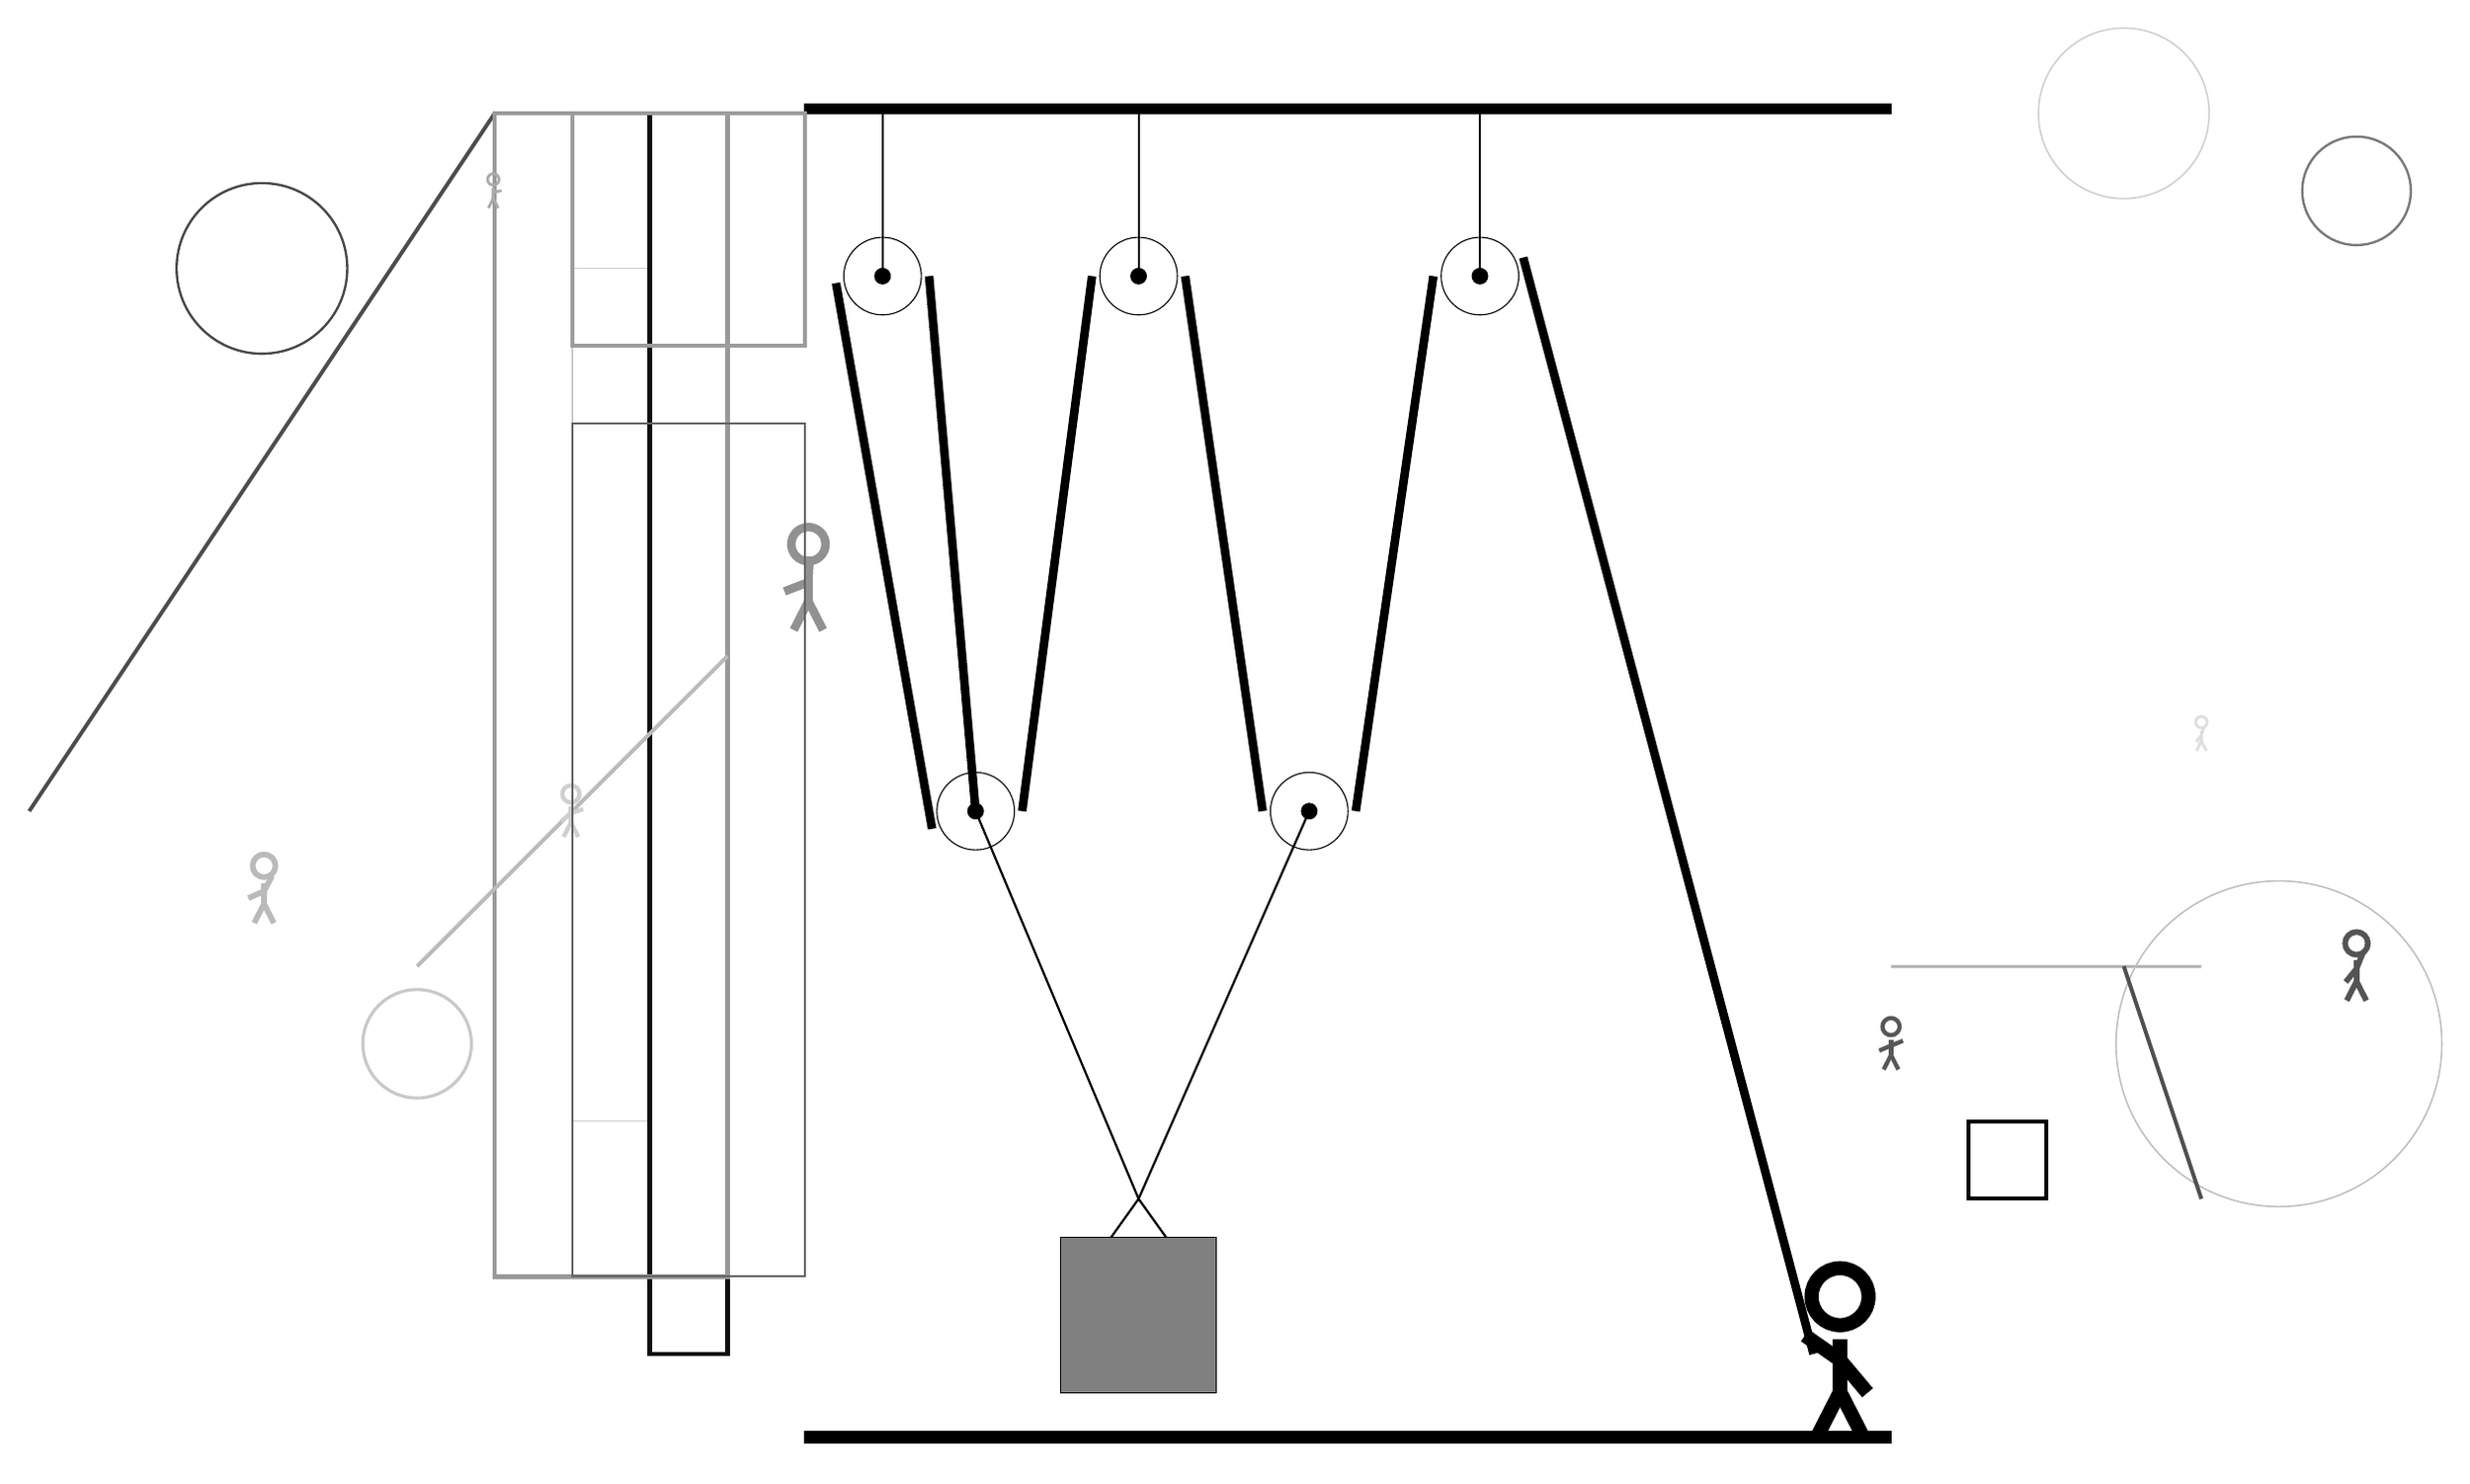
\begin{tikzpicture}
			%%%%% START %%%%%
			
			\draw[fill=black] (-2, 14) rectangle (12, 14.125);
			
			\draw (-1, 11.9) circle (0.5);
			\draw[fill=black] (-1, 11.9) circle (0.1);
			\draw[thick] (-1, 11.9) -- (-1, 14);
			
			\draw[line width=0.4mm, color=black!29] (12, 3) rectangle (16, 3);
			
			\draw[line width=0.5mm, color=black!70](-6, 14) -- (-12, 5);
			\draw[line width=0.2mm, color=black!20] (-4, 12) rectangle (-5, 1);
			\draw [line width=0.3mm, color=black!53](18, 13) circle (0.7);
			\node[line width=0.5mm, color=black!27] at (-9, 4) {\Strichmaxerl[4][24][62]};
			\node[line width=0.5mm, color=black!43] at (-2, 8) {\Strichmaxerl[6][21][87]};
			
			\draw [line width=0.3mm, color=black!72](-9, 12) circle (1.1);
			
			\draw[line width=0.6mm, color=black!94] (-3, 14) rectangle (-4, -2);
			\draw[line width=0.6mm, color=black!40] (-3, -1) rectangle (-6, 14);
			\draw[line width=0.5mm, color=black!27](-3, 7) -- (-7, 3);
			\draw [line width=0.2mm, color=black!25](17, 2) circle (2.1);
			\node[line width=0.3mm, color=black!67] at (18, 3) {\Strichmaxerl[4][51][68]};
			\node[line width=0.7mm, color=black!66] at (12, 2) {\Strichmaxerl[3][23][22]};
			
			\draw[line width=0.5mm, color=black!69](15, 3) -- (16, 0);
			\node[line width=0.2mm, color=black!19] at (-5, 5) {\Strichmaxerl[3][41][17]};
			\draw[line width=0.5mm, color=black!39] (-2, 11) rectangle (-5, 14);
			\draw [line width=0.4mm, color=black!21](-7, 2) circle (0.7);
			\node[line width=0.2mm, color=black!33] at (-6, 13) {\Strichmaxerl[2][85][9]};
			\draw [line width=0.2mm, color=black!19](15, 14) circle (1.1);
			\draw[line width=0.5mm, color=black!99] (14, 1) rectangle (13, 0);
			\draw[line width=0.3mm, color=black!61] (-2, -1) rectangle (-5, 10);
			
			\node[line width=0.3mm, color=black!13] at (16, 6) {\Strichmaxerl[2][55][71]};
			
			\draw (2.3, 11.9) circle (0.5);
			\draw[fill=black] (2.3, 11.9) circle (0.1);
			\draw[thick] (2.3, 11.9) -- (2.3, 14);
			
			\draw (6.7, 11.9) circle (0.5);
			\draw[fill=black] (6.7, 11.9) circle (0.1);
			\draw[thick] (6.7, 11.9) -- (6.7, 14);
			
			\draw (0.2, 5) circle (0.5);
			\draw[fill=black] (0.2, 5) circle (0.1);
			
			\draw (4.5, 5) circle (0.5);
			\draw[fill=black] (4.5, 5) circle (0.1);
			
			\draw[thick] (0.2, 5) -- (2.3, 0)  -- (4.5, 5);
			\draw[thick]  (1.8, -0.7) -- (2.3, 0) -- (2.8, -0.7);
			\draw[fill=black!50] (1.3, -0.5) rectangle (3.3, -2.5);
			
			\draw[line width=1.1mm] (0.2, 5) -- (-0.4, 11.9);
			\centerarc[line width=1.1mm](-1, 11.9)(0:200:0.6);
			\draw[line width=1.1mm] (-1.6, 11.81) -- (-0.361, 4.772);
			\centerarc[line width=1.1mm](0.2, 5)(200:360:0.6);
			\draw[line width=1.1mm](0.8, 5) -- (1.7, 11.9);
			\centerarc[line width=1.1mm](2.3, 11.9)(0:180:0.6);
			\draw[line width=1.1mm] (2.9, 11.9) -- (3.9, 5);
			\centerarc[line width=1.1mm](4.5, 5)(180:360:0.6);
			\draw[line width=1.1mm] (5.1, 5) -- (6.1, 11.9);
			\centerarc[line width=1.1mm](6.7, 11.9)(20:180:0.6);
			\draw[line width=1.1mm](7.258, 12.14)  -- (11, -2);
			
			\node at (11.3, -2) {\Strichmaxerl[10][-35][-50]};
			
			\draw[fill=black] (-2, -3) rectangle (12, -3.15);
			
			%%%%% END %%%%%
		\end{tikzpicture}
	\end{figure}	
\end{document}